\chapter{Biological Background}\label{chapter:biology}

Sounds\dots{} For sure, they are one of the most important sources of information in our everyday life. By listening to them, one can describe what is happening around, understand how to react to occurring situations, or even tell if a danger is approaching, and it is time to take action. It is hard to imagine human sensation without hearing, but as easy as this may sound (no pun intended), the~biology behind it is quite complicated. This chapter will introduce the reader to how sound as a~mechanical phenomenon is converted to sound as perception and provide a~basic overview of the structures in the human ear, along with the mechanical and neurobiological processes happening inside of them.

\section{Outer and Middle Ear}

At the beginning, sound approaches the ear by vibrations in the air (or any other elastic medium) and enters the outer ear, which consists of the visible part (called the auricle, or the pinna) and the ear canal. The auricle is a thin plate of elastic cartilage, covered with integument, and connected to the surrounding parts by ligaments and muscles; and to the beginning of the ear canal by fibrous tissue. The ear canal is a tube leading from the~bottom of the~auricle to the middle ear, separated from it by the eardrum (or tympanic membrane). The main purpose of the ear canal is to focus the sound energy gathered by the auricle on the~eardrum. It also amplifies frequencies between 3\,kHz and 12\,kHz \cite{Standring2008}.\\

Being gathered on the eardrum, the mechanical vibrations propagate through the middle ear. Three bones (called the ossicles) are located inside of it. The malleus (also called the hammer) is connected to the eardrum and transfers the vibrations from it to the incus (the anvil). These vibrations are chaotic, but the malleus is connected to the eardrum in a linear manner, helping the ear to respond more linearly and smoothly. The incus, in turn, connects to the stapes (the stirrup). The footplate of the stapes introduces pressure waves in the inner ear, which starts with the oval window of the cochlea. The structures of the middle ear can be seen on figure~\ref{img:anatomy_human_ear}.\\

It may sound redundant to have additional structures in the ear which propagate the vibrations even further, when they could travel just one centimeter more in a way like before, in the ear canal, but in reality, the pressure of these mechanical vibrations is too small to cause the waves of the same velocity in the cochlear fluids. The ossicles help to amplify the pressure of these vibrations. They are positioned to form a lever, and, because the oval window is about 14~times smaller than the eardrum, the pressure gain becomes quite significant in the end -- at~least 18.1~times \cite{Standring2008}.

\begin{figure}[h]
	\centering
	\begin{subfigure}{0.5\textwidth}
		\centering
		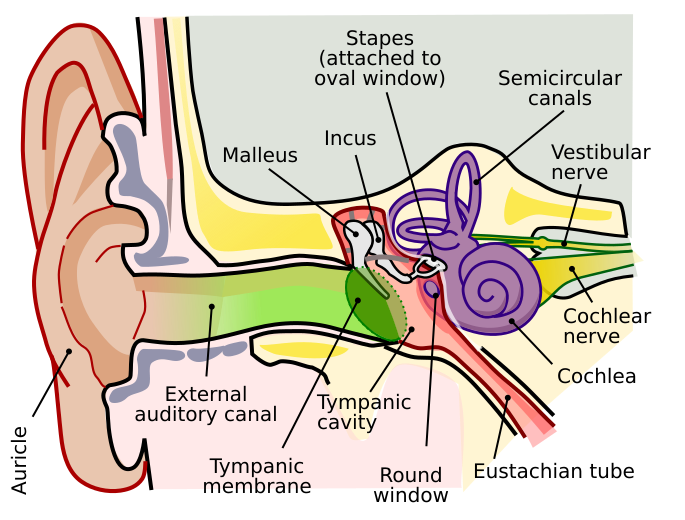
\includegraphics[width=\linewidth]{include/anatomy_of_the_human_ear}
		\caption{}
		\label{img:anatomy_human_ear}
	\end{subfigure}%
	\begin{subfigure}{0.5\textwidth}
		\centering
		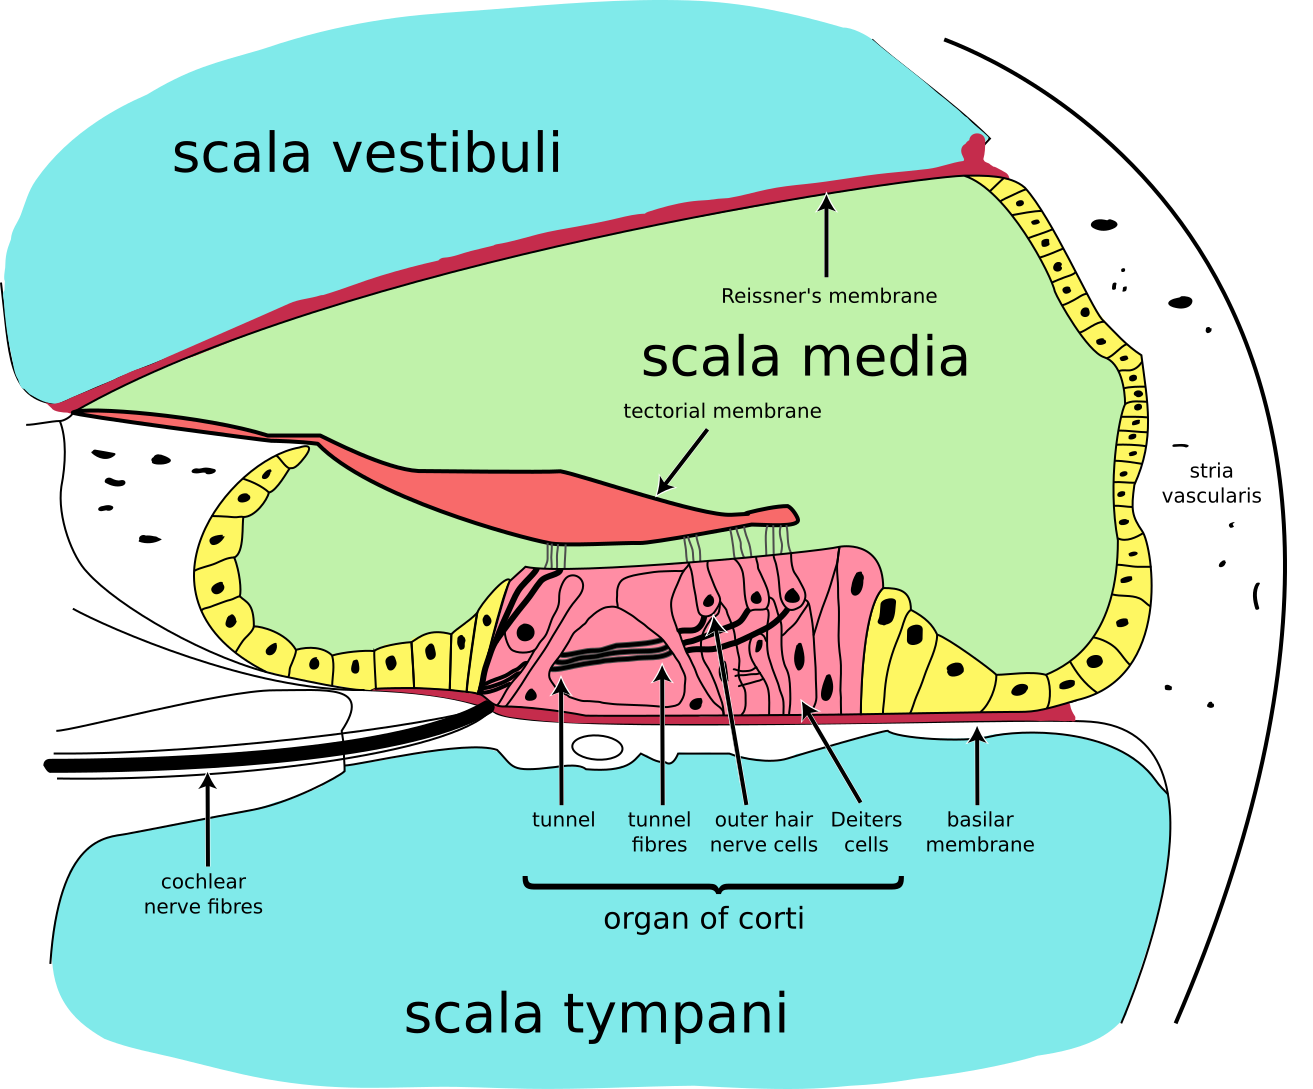
\includegraphics[width=\linewidth]{include/cochlea_cross_section}
		\caption{}
		\label{img:cochlea_cross_section}
	\end{subfigure}
	\caption[Anatomy of the human ear]{\textbf{(a)} Anatomy of the human ear. The ossicles of the middle ear are shown in white. The inner ear is shown in purple. \textbf{(b)} Cross-section of the cochlea showing the organ of Corti and three chambers filled with cochlear fluids. Both pictures were taken from \url{{https://commons.wikimedia.org/}}}
\end{figure}

To regulate the middle ear and protect it from damage due to very loud sounds, two muscles are located inside of it: the stapedius muscle and the tensor tympani muscle. These muscles are controlled by unconscious reflexes and hold the ossicles when the vibrations become too intense. To provide ventilation and drainage of the middle ear and to equalize pressures in this isolated environment, the middle ear is connected to the back of the throat by the eustachian tube \cite{Schnupp2011}.

\section{Inner Ear}

The inner ear starts with the above-mentioned oval window, which is connected to the stapes of the middle ear. The oval window is a part of the cochlea –- a structure of the inner ear dedicated to hearing. Along with the cochlea, the inner ear also contains the vestibular system, which is responsible for the sense of balance and spatial orientation and uses the same kinds of fluids and cells as the cochlea does. The vestibular system will not be covered in this thesis, but the fluids and cells will be described in more detail later in the section.\\

The cochlea itself is a spiral-shaped cavity made of bony tissue, which makes about 2.75~turns around its axis and is about 3\,cm long. The core component of it is the basilar membrane, which runs along almost its entire length and separates two of the three chambers of the cochlea filled with different fluids \cite{Schnupp2011}: the tympanic duct (scala tympani) filled with perilymph, and the cochlear duct (scala media) filled with endolymph. The third chamber, the vestibular duct (scala vestibuli), is separated from the cochlear duct by the Reissner’s membrane and is filled with perilymph (figure~\ref{img:cochlea_cross_section}). When the footplate of the stapes of the middle ear introduces movements to the cochlear fluids, the basilar membrane is affected too, and the endolymph in the cochlear duct moves along.\\

The most interesting property of the basilar membrane is that its stiffness and width is different throughout its length – the membrane is narrow and stiff at the basal end of the cochlea, and wide and floppy at the apical end. And here sound waves have two possible routes to take while propagating through the basilar membrane: a shorter path, which includes going through the stiffer parts of it, or a longer path, which means travelling along the membrane until it becomes easier to pass through, but pushing more fluid on the way. In fact, high-frequency waves tend to choose the shorter path, and low-frequency waves – the longer one. The scale between frequencies passing through the basilar membrane is not linear, but close to logarithmic. In machine hearing systems, equivalent rectangular bandwidth (ERB) scale is usually used.\\

Thus, the basilar membrane moves in different places depending on the frequencies of the vibrations. The organ of Corti, which sits on top of it and runs along its entire length, contains displacement cells able to detect movements of the fluid nearby and excite the nearby neurons to send electrical impulses. Such cells are packed with a bunch of stereocilia (hair) that stick out of its top, and thus are called hair cells. These cells can be of two types: inner hair cells that are located closer to the center of the cochlea, and outer hair cells that sit closer to its outer side. Inner hair cells are less numerous than outer hair cells and form a single row along the organ of Corti, while outer hair cells usually form three rows \cite{Schnupp2011}.\\

Now, it is important to mention that the endolymph in the cochlear duct contains high amounts of positively charged ions (primarily potassium and calcium). When it moves in response to the sound pressure, the stereocilia of the inner hair cells are deflected, and tiny ion channels open in them. This allows the charged ions from the endolymph to enter the stereocilia. The cell becomes depolarized, and a receptor potential is produced. This results in releasing the neurotransmitters at the basal end of the cell and then triggering action potentials in the nerve nearby. In this way, inner hair cells detect movements around them and convert mechanical sound waves to electrical nerve signals.\\

Outer hair cells, in turn, serve as amplifiers of the quiet sounds. Their receptor potentials are converted to cell body movements, thus increasing the sound pressure \cite{Hudspeth2008}.

\section{Auditory Scene Analysis}\label{section:biology_asa}

To close up the chapter, it was decided to make an introduction to auditory scene analysis according to Bregman \cite{Bregman1990}. His book named \textit{"Auditory Scene Analysis: The Perceptual Organization of Sound"} (1990) made a big influence on further researches, as it attempted to bring together the theoretical knowledge in the field, which did not have any clear base to build on. Bregman's book is now widely recognized as this base, so it is necessary to list at least the primary concepts of ASA described there. This section could have been put to either of the chapters in the theoretical part of the thesis, because it is connected to every field being discussed, but it resides in the biological part, because most of the addressed experiments were testing human auditory perception and are highly connected to the related studies in Gestalt psychology.\\

To start off, Bregman brings to the world a new term related to auditory perception. If you recall the two definitions of sound from chapter \ref{section:physics_sound}, you may remember that there were two of them: one related to sound as a physical phenomenon, and another related to perception in the brain. Bregman introduced a term "auditory stream", or "auditory object" to address the second definition. He made an analogy with vision and how humans tend to group separate surfaces of the same object on their eye retina to see this object as a whole and referred to "auditory streams" as to the same kind of objects, but for audition. He said that the term "sound" is not really well suitable in this case, because for example a melody in a recording of music consists of different sounds (notes), but people often percept this melody as a whole and group the sounds into something greater in their perception. Bregman's definition of auditory streams became very popular, so it will be used throughout this thesis too.\\

Bregman defines ASA as the process of separating these auditory streams from mixtures and refers to it as to a two-stage process. The first stage (segmentation) is said to be splitting the auditory input into so-called "segments", just as the visible object is split into surfaces in the human eye. The second stage is grouping and refers to integrating these segments together based on the grouping cues. With references to experiments from his lab he describes two possible approaches to grouping and searching for cues: simultaneous (which is also called vertical, or spectral) and sequential (or horizontal). While simultaneous grouping takes into account the segments that appear at the same time, but relate to different frequencies (are spread in space), sequential grouping works with segments that share the frequency component, but are located at different points in time. As an example of a cue for simultaneous grouping one could take common onset and offset, because it is usual for sounds (or different frequency components of the same sound) from the same source to start at the same time. For sequential grouping, probably the most common cue is pitch. If two sounds have pitches associated with fundamental frequencies that are close to each other, the sounds will likely be grouped to the same stream. When the frequencies are further away, the sounds will most certainly appear in different streams.\\

For a demonstration of sequential grouping, consider a galloping sound that consists of two alternating tones: "A-B-A". The pattern repeats endlessly with a variable speed. The fundamental frequencies of the tones A and B can also be varied. Experimentally \cite{Schnupp2011} it was discovered that when the fundamental frequencies are close to each other and/or the speed of repeating the pattern is small, there is only one resulting stream in the perception of the sequence. On the other hand, when the frequencies are further away and/or the sequence is being repeated at a faster rate, the subjects report that they can hear two streams: one consisting of repeating A sounds ("A-{}-{}-A-A-{}-{}-A"), and another of repeating B sounds ("-{}-B-{}-{}-{}-{}-B-{}-"). The subjects also reported that they can only focus their hearing only on one of the two streams, and the other one was heard in the background. Interestingly, when the repeating rate and the difference in frequencies were set to some specific values, the subjects reported that the perception of two streams was alternating with the perception of one stream every 15-20~seconds. This phenomenon was experimentally verified during the research for this thesis with the help of the website made for \cite{Schnupp2011}.\\

In his book \cite{Bregman1990}, Bregman described a similar experiment, but the repeating pattern was more complex. There were six tones: three lower ones (1,~2~and~3) and three higher ones (4,~5~and~6), and they were repeating in a pattern like this: "1-4-2-5-3-6". Bregman asked the subjects to report the order of the heard tones, and at faster rates of repeating they were failing to do this for both groups at the same time. When they were focusing the hearing on the lower tones, the higher ones were heard in the background, and thus it was difficult to correctly determine the order.\\

As an example for simultaneous grouping, Bregman makes another experiment. This time, the pattern consists of two alternating sounds: a pure tone (A) and a complex tone that consists of two pure tones (B and C). Again, the pattern repeats endlessly, and both the speed of repetition and fundamental frequencies of the tones might be changed. As a result, Bregman reports that the tone B was \textit{"an object of rivalry"} (\cite{Bregman1990}, p.654): in cases when A was close to it in frequency, they were grouped together in a simultaneous manner, but when they were further away from each other, the tone B was rather grouped simultaneously with C, thus creating a richer tone BC.\\

Bregman's theory is highly related to the studies in Gestalt psychology. He was drawing parallels between vision and hearing, and found a lot of similarities between them that were supported by the Gestalt laws of grouping. He described the concepts of "belongingness" and "exclusive allocation", and the principles of similarity, proximity and closure. Also, he was questioning whether scene analysis is an innate process, or the one acquired by learning.\\

Finally, to make a parallel with computer modeling, Bregman referred to the notion of heuristics. In his words, heuristics are \textit{"the procedures that are not guaranteed to solve the problem, but are likely to lead to a good solution"} (\cite{Bregman1990}, p.\,32). He believed that outputs from multiple heuristics should be used at the same time to find this good solution, and that there are similar mechanisms in human perception. For example, when there is evidence about common onsets and offsets of two frequency components of a sound, and it was supported by the fact that these components were different harmonics of the same fundamental frequency, the probability of being incorrect after guessing that these components should be grouped in the same stream becomes really close to zero. Here, the two heuristics contributed to the decision of whether to group the sounds into a single stream.\\


